\documentclass[10pt]{article}
\usepackage[a4paper,margin=17mm]{geometry}
\usepackage{amsmath,amssymb,graphicx,hyperref,booktabs}
\hypersetup{colorlinks=true,urlcolor=blue}
\setlength{\parindent}{0pt}\setlength{\parskip}{5pt}
\begin{document}
\begin{center}\Large Saturated-yield scaling and the parameter gap\\[3pt]
\normalsize 16 November 2026 --- numeric models, PCC unverified\end{center}
The proposed six-summand balance needs a fresh admissibility/size analysis.
The existing bound exceeds its unit-constant target size. This is
a scoped model/arithmetic result, not an algorithmic lower bound.
PCC-20261116-ebfd31 and76dc04. [pcc:unverified]

\textbf{Conditional model.} Let $B=N^\beta$, $m$ be fixed arity, and suppose
$y=\Theta(\min(1,B^m/N))$, $D=\widetilde O(B^\gamma)$, setup and sparse
kernel cost $\widetilde O(B^2)$, with all other phases charged on an admissible
growing family. The proposed cost $P+BD/y+L$ has envelope
\[
E(\beta)=\max\{2\beta,(1+\gamma)\beta+\max(0,1-m\beta)\}.
\]
These algorithmic and distribution assumptions are unproved. [pcc:unverified]

\begin{center}
\begin{tabular}{ccccc}\toprule
$m$&Hypothetical $\gamma$&Candidate $\beta$&Model exponent&Evidence\\\midrule
4&$1/2$&$2/9$&$4/9$&Rational Lean endpoints\\
5&$3/2$&$1/5$&$1/2$&Native model only\\
6&$3/2$&$1/6$&$5/12$&Rational Lean endpoints\\
8&$5/2$&$1/8$&$7/16$&Native model only\\\bottomrule
\end{tabular}\end{center}
For the six-sum row, the uncapped balance $\beta=2/11$ suggests $4/11$;
the capped model there is $5/11$. Its rational minimum is $5/12$ at $1/6$.
The gate audits 12 declarations, ten named endpoints, with zero failing or
trusted-native axioms. No actual decomposition complexity follows.
PCC-20261116-76dc04. [pcc:unverified]

\begin{center}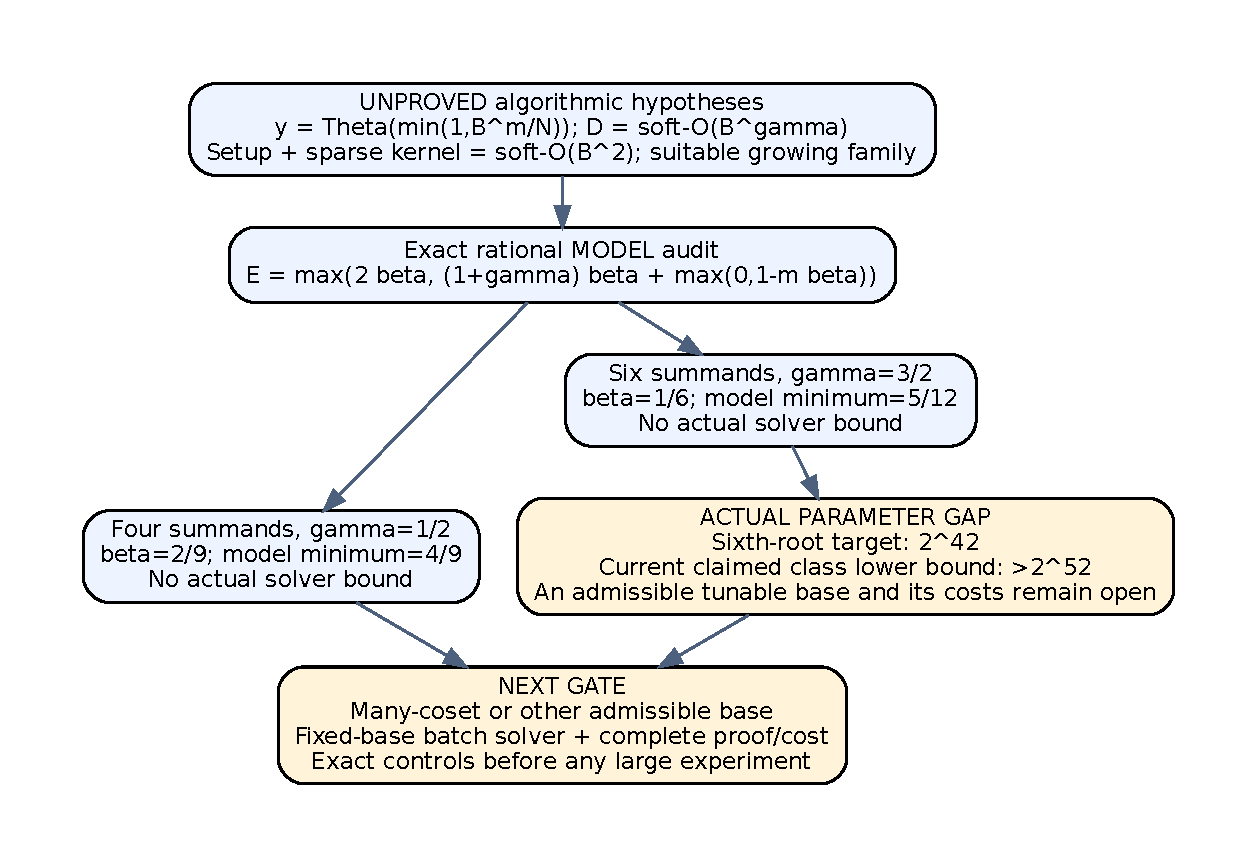
\includegraphics[width=0.96\linewidth,height=105mm,keepaspectratio]{pipeline.pdf}\end{center}
\newpage
\begin{center}\Large Actual parameters and the revised execution gates\end{center}
\textbf{Integer audit.} At the actual scalar-order integer
$N=2^{252}+27742317777372353535851937790883648493$,
\[
\lfloor N^{1/6}\rfloor=2^{42}=4398046511104.
\]
The current $M=12965132697890207$ and earlier transport bound give
$B\ge(M-1)/2=6482566348945103$. Both the fifth and sixth powers of that
lower-bound integer exceed $N$. Four Core proofs check these integer facts;
they do not certify the transport premise or a point count. Reusing the old
base cannot certify the intended finite six-sum balance with the stated
unit-constant budget. This is not a calibrated runtime comparison or an
exclusion of other bases, solvers or asymptotic parameter paths.
PCC-20261116-76dc04. [pcc:unverified]

\textbf{Arithmetic-only candidates.} The audit proposes the following raw products:
\begin{center}\begin{tabular}{rrr}\toprule
Subgroup order&Cosets&Proposed raw cardinality\\\midrule
213156431&20633&4398056640823\\
60824497&72308&4398097729076\\\bottomrule
\end{tabular}\end{center}
Coset distinctness, sign-alias exclusion, point transport, normalized base
size, recognition cost and growing-family availability are unchecked.
Thousands of branches do not inherit the four-coset compiler cost.
Two exact Rust controls pass, including rational-grid comparison. The
immutable executable was hashed before calls; the source archive is marked
post-call. No sampling, solver or timing experiment was run.
PCC-20261116-ebfd31. [pcc:unverified]

\textbf{Revised sequence.}
\begin{enumerate}
\item Freeze cost/admissibility cards for four, five and six summands;
include finite constants, memory, success law, every failed query and setup.
\item Resolve base-size availability and recognition cost first. Investigate
four-sum sublinear-query and six-sum subquadratic-query algorithms only at
parameters that actually meet their hypotheses.
\item Batch targets within one DLP and one common factor-base column universe.
Explore structured elimination and modular composition; charge coefficient
expansion and root discovery in every multipoint-evaluation proposal.
\item Review and formalize geometric energy, actual-point and hidden-tag
selection bridges. The existing four-sum draft does not supply six-sum yield.
Bounded restarts remain a conditional proposal; quadratic-RAM birthday
diagnostics are separate. PCC-20261116-f0439a. [pcc:unverified]
\item Compare actual Edwards-y, Montgomery and selected quotient presentations
on identical instances. Any twist/isogeny proposal supplies explicit DLP
transport and its complete cost.
\item Exact controls, then preregistered qualified native comparisons, then
six sizes across 24 order bits and held-out predictions. Runner/cost admission
is still required. A measured slope alone is not an asymptotic proof.
\end{enumerate}

\textbf{Rejection scope.} Use frozen ROUTE\_CRITERIA\_V3: mathematical
exclusion, exact counterexample, corrected rejection of a finite promise,
implementation parked, invalid experiment, or open. A timeout does not prove
a universal exponent lower bound. No measured-performance graph changes.

\textbf{Sources.} Source-linked REPORT.md and the adjacent proof maps/receipts
give scope and reproduction details.
\href{https://people.maths.ox.ac.uk/petit/files/16PKC_primeECDLP.pdf}{PKM2016, sections3.1--3.2};
\href{https://arxiv.org/html/2205.00342v1}{Bhargava et al., coefficient input/Theorem1.1};
\href{https://users.cs.duke.edu/~elk27/bibliography/91/KaSa91.pdf}{Kaltofen--Saunders, section4}.
KB unavailable; bounded repository and primary-source fallback. The Edwards
symmetry eprint returned403. No novelty clearance or new attack-exponent claim.
[pcc:unverified]
\end{document}
